\graphicspath{{included-papers-tex/paper-4/figures/}}

\includedPaper{\textsc{paper iv - perceived behaviors of personality-driven agents}}{\textsc{paper iv - perceived behaviors of personality-driven agents}}{Alberto Alvarez and Miruna Vozaru}

\normalfont
% \textbf{\textsc{ABSTRACT}}

% We propose modeling designer style in mixed-initiative game content creation tools as archetypical design traces. These design traces are formulated as transitions between design styles; these design styles are in turn found through clustering all intermediate designs along the way to making a complete design. This method is implemented in the Evolutionary Dungeon Designer, a research platform for mixed-initiative systems to create roguelike games. We present results both in the form of design styles for rooms, which can be analyzed to better understand the kind of rooms designed by users, and in the form of archetypical sequences between these rooms. We further discuss how the results here can be used to create style-sensitive suggestions. Such suggestions would allow the system to be one step ahead of the designer, offering suggestions for the next cluster, assuming that the designer will follow one of the archetypical design traces.

\textbf{\textsc{PUBLISHED IN}}

Violence | Perception | Video Games: New Directions in Game Research, [transcript], 2019

%\section*{PERCEIVED BEHAVIORS OF PERSONALITY-DRIVEN AGENTS}

\section*{PERCEIVED BEHAVIORS OF \\ PERSONALITY-DRIVEN AGENTS}

\subsection{Introduction}

The discussion regarding the believability of video game characters in the fields of game analysis and artificial intelligence research has taken many forms over the years, generally focusing on appearance and behavior~\citepfourth{p4Lankoski2007-GameplayDesignPatterns,p4Umarov2012-BelievableAI,p4Lee2012-BelievableCharacters}. In the paper at hand, we will present a study in which we chose to focus on behavioral believability.

The pervading notions related to the degree of character believability seem to be their awareness, reaction capabilities, and adaptability to the events taking place around them~\citepfourth{p4Warpefelt2014-BelievabilityNPC}. These factors seem to be connected to the mental schemas activated by the visual depictions of characters and the game world~\citepfourth{p4Stein92-SchemasCognitiveScience}. This made us question how the believability of an agent would be affected by the absence  of anchoring references. Stripping away referential visual depictions, narrative, and the relevance of affordances to the traversal of the game world, we sought to understand the narratives that observers create around an ambiguous entity acting within an abstract environment.

In this paper, we will first present our reasoning and the theoretical background of the research design, the technical aspects of the AI agent that served as our character, and the responses that participants provided following the viewing of several films depicting the actions of the agent. Finally, we will discuss our conclusions and implications for future research and game development.


\subsection{Theoretical Background}

The purpose of this research is to analyze the means through which the viewer makes sense of ambiguous behavior in the absence of corresponding mental schemas. To do this, we needed to understand the means by which information is perceived and integrated, and what the observer uses to fill in the blanks when the stimulus is too ambiguous to fit into pre-existing information. New information, such as that presented by the behavior of an observed game character, is integrated within the pre-existing mental schemas of the observer, which are used to shape the meaning of the new information and make predictions about future developments. For instance, in the video game PORTAL~\citepfourth{p4portal}, the portal gun activates the mental schemas corresponding to previously encountered guns in video games. Namely that it can shoot, it is a tool for progressing in the game, and it damages enemies. When the portal gun is used, instead of damaging an enemy, it creates a gateway that the player can use to traverse the game. This result does not match pre-existing knowledge, which will force a schema modifi- cation concerning the video game gun functionality. The visual representation affords the integration of the portal gun within the player’s previously acquired knowledge; it is referential, descriptive, and concrete. The differences become apparent once the observed functionality does not match expected performance.
 
Affordance theory, popularized in design by Donald Norman, describes the action and use possibilities that an entity, object, or environment possesses~\citepfourth{p4Norman2002-DesignEverydayThings}. This theory has been widely appropriated by game design, due to the designer’s needs to communicate briefly, clearly, and coherently the means through which a player can traverse a game. Affordances can be tied to previously acquired knowledge, but also be assigned meaning derived strictly from their application within the game world. They are used to telegraph the ways in which the players can use the different elements at their disposal to navigate the game world and to constrain the situational role of the elements.

That being said, the perception of use and role is not a necessary factor in the perception of agency and attribution of specific behaviors. In a study conducted by Heider and Simmel, participants were shown a brief video in which the actors were a circle, a large triangle, and a small triangle~\citepfourth{p4Heider44-ApparentBehavior}. The shapes were depicted in various types of motion, seemingly interacting with each other and the environment. The participants were then prompted to describe the events taking place in the video. All of the participants, with the exception of one, described the events of the video as part of a narrative, whether it was as two parents fighting in front of their child, or two people finding themselves in a romantic situation and then being interrupted by a third. This led us to conclude that the perception of self- directed motion transforms the interpretation of a pattern into one involving an agential entity~\citepfourth{p4Harris2011-AbstractMotion}.

So far, we can conclude that the believability of the agent hinges on its recognizable visual representations, as well as the affordances displayed within the game world. By stripping these factors and endowing a visually ambiguous object with self-directed motion, it will be interpreted as an entity with perceived agency.

Personality traits have generally been viewed as probabilistic determinants for the predictability of a certain type of behavior mediated and moderated by  the current situation~\citepfourth{p4McCrae92-fiveFactorModel,p4Mischel95-TheoryPersonality,p4Tett2000-SituationTrait,p4Costa1998-TraitTheoriesPers}. The Cybernetic Big 5 model, henceforth CB5T, treats personality-endowed agents as goal-based entities perpetually engaged in goal attainment loops~\citepfourth{p4Deyoung2015-CyberBigFive}. The goal loops are divided into stages, with personality traits exerting their influence on each stage of the loop. Traits are manifested through characteristic adaptations, which, unlike personality, are constructed based on individual life experiences and are thus not universal. For instance, the manifestation of the trait compassion can take different characteristic adaptations, such as volunteering or monetary donations, which are dependent on the individual’s socio-cultural environment.

While our intentions steer clear of transforming the research into a projective test\footnote{A projective test is a psychological assessment during which participants are asked to interpret ambiguous stimuli with the assumption that the interpretation will reveal insights regarding their personality traits}, we decided to use personality factors as behavior determinants for our AI agents. Our hypothesis was that in the absence of other anchoring visual primers, the observers would integrate the perceived behavior within familiar characteristic adaptations. While we used Heider and Simmel’s experiment as a starting point, our research was also informed by the similarity-attraction hypothesis, which states that individuals grant more positive appraisals to responses that match their own personality traits~\citepfourth{p4Byrne67-AttractionSimilarity}. The agents were given the same traits as the corresponding observer. We used an AI agent instead of a pre-rendered movie, due to the options it offered in terms of personality customization. We distinguish our purposes from the creation of narratives surrounding ambiguous agents. To clarify, our purpose was not the exploration of the participants’ creation of narratives surrounding the ambiguous behavior of an agent, but to explore the participants’ propensity to recognize behaviors with which they are most familiar – the ones they have observed in themselves.

\subsection{Agent Behavior and Design}

The following section will cover the psychological and visual design of the AI agent, its personality, emotions, and affective behavior, as well as the reasoning behind the aesthetic choices we made.

As mentioned above, the CB5T model moves away from previous models and classifies traits as global influencers of the goal attainment loop, which is broken down into five stages: goal activation, action selection, action, outcome interpretation, and goal comparison. As a result of the ongoing process of receiving, perceiving, and filtering environmental stimuli, multiple goals can be active at the same time. The first and second phases are internal and generally com- prised of parallel processes. The third phase presents a bottleneck to the goal loop, due to the fact that, while a person can hold multiple goals in their memory at the same time, actions are generally performed in sequence. In the fourth phase, the result of the action is measured against the intended results, which  will generate a match or a mismatch. This will in turn inform the next goal and the subsequent cycle. Personality traits exert their influence in concert at every stage of the goal loop, becoming moderators to the goal attainment stages. For a better understanding of the goal loop, we can consider the following situation: The AI agent feels hungry, and in the process of trying to obtain food it realizes that it must jump over an obstacle. While both goals exist in its memory, the fact that it can perform only one action at a time determines that it must first perform the jump. This is the action selection phase. The agent jumps and fails to over- come the obstacle. The actual result and the intended result do not match, and its personality score will influence its reflection on this failure.

The CB5T model was coupled with a simplified version of the  Ortony, Clore, and Collins model of emotions (henceforth OCC), “The OCC model revisited.~\citepfourth{p4Steunebrink2009-OCCModelRevisit}” The reasoning behind the combination of personality and emotion models was derived from the need to visually depict the results of the internal processes taking place during the goal attainment phases. The influence exerted by personality traits on the goal attainment loop materializes in affective behavior, where the emotional valence and intensity is dependent on the personality score.

\begin{figure}[ht!]
\centerline{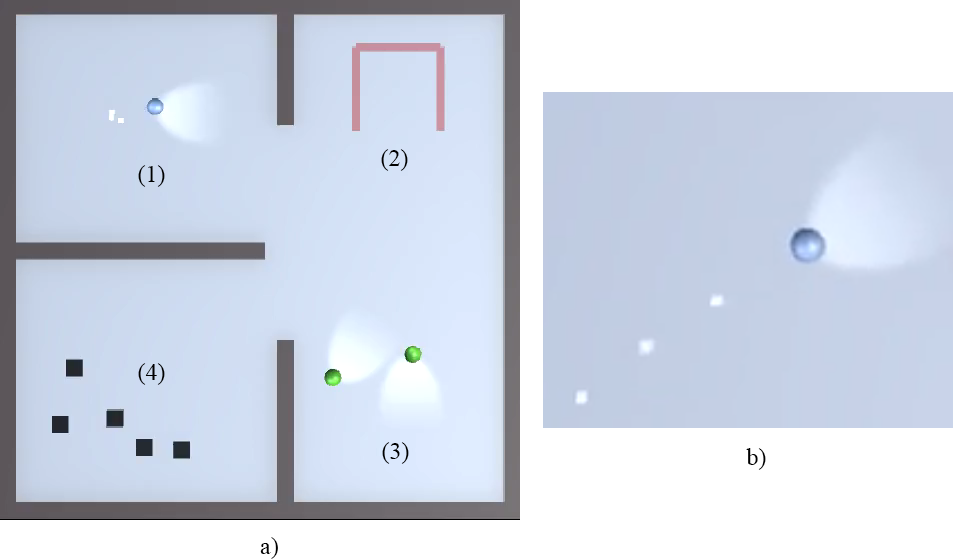
\includegraphics[width=0.8\textwidth]{figure-1-composed.png}}
\caption{Simulation environment.(a) Example environment that was presented to users, containing the personality-driven agent (1), and three different situations that the agent will encounter (2,3,4). (b)	Agent trail and view.}
\label{figs:env-agent}
\end{figure}


Intentionality and attention presented a large part of the concretization of personality-derived behavior. The agent’s attention and intentions were depicted by a cone of light in front of it, maintaining the ambiguity of the stimulus but strengthening the perception of agency. Similarly, the trail the agent leaves be- hind signifies its movement speed which is dependent on its emotional arousal. The affective behavior exhibited by the agent had to be contextualized in specific situations, in order to be granted environmental referentiality. We created several situations, including but not limited to: positive and negative social situations, environmentally challenging situations, and situations that could produce distractions.

\subsection{Agent Architecture and Simulation}

Human-like behavior is a complex subject and one that cannot be approached by using only one model or technique. Rather, different approaches use a compendium of specialized modules. For instance, emotional, personality, memory, or social modules that have various responsibilities in order to simplify the decision-making process.

The TOK architecture represents an agent as a set of different modules that handle the perception, reactivity, goals, emotions, and social behaviors. TOK is divided into three main components: (1) HAP, the goal-based reactive engine, (2) EM, the emotional model, and (3) Glinda, the natural language system~\citepfourth{p4Bates94-architectureAES}.

\begin{figure}[ht!]
\centerline{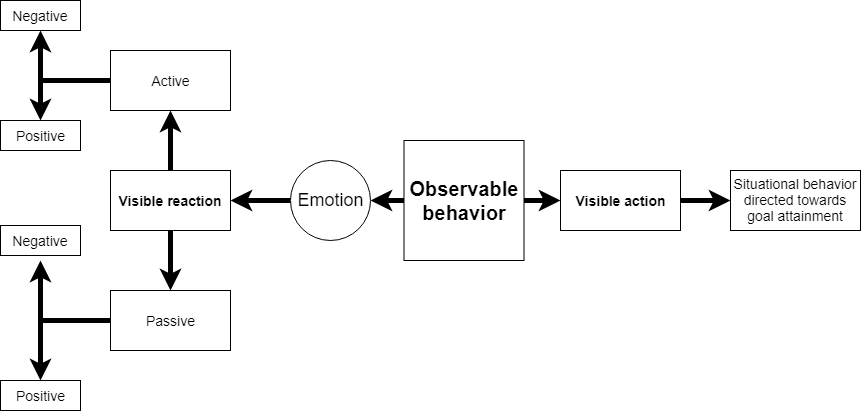
\includegraphics[width=\textwidth]{big-figure.png}}
\caption{Observable Behavior. The observable behavior by the users is based on the set of actions provided by the encountered situation, which results in an emotional reaction. The reaction is based on the outcome interpretation phase, where the agent will choose the respective emotion (active/passive and negative/positive), intensity and reactive behavior.}
\label{figs:observableBehavior}
\end{figure}

Our model assimilates to HAP and EM, in that HAP selects an action based primarily on the agent’s goals, emotions and perception by using the CB5T model, and with EM it calculates the emotional valence of the agent by comparing environmental stimuli with goals, possible actions with standards, and environmental objects with attitudes.

The agent’s goals have a dynamic weight and a priority. The weight is determined by the agent’s moment-to-moment actions and reflect its progression and perception of environmental cues. The priorities indicate the goal type, and their influence on survival and self-actualization. To exemplify, “hunger” is a priority 1 goal, and its weight will increase according to the presence of food in the agent’s proximity and the time they spend roaming around the environment.

Subsequently, according to the outcome of the situation, the agent will feel pleased or displeased in accordance with the match or mismatch between the desired outcome and the actual one. The combination of the outcome difference and the personality traits trigger different emotional reactions. As presented in figure~\ref{figs:observableBehavior}, the agent can perform several actions in specific situations and the con- sequence of the selected action entails not only different emotions but also different levels of arousal.

\newcolumntype{Y}{>{\centering\arraybackslash}X}
\begin{table*}[ht]
% \centering
\caption{Reaction table used to choose the respective emotional reaction. First, we choose the agent’s emotion by choosing if active/passive and negative/positive  as presented in figure 2, with the addendum that if more than one option is viable, the choice will be based on the situation’s target. Finally, the intensity is calculated.} \label{p4tab:reactionTab}
% \resizebox{0.8\textwidth}{!}{
\centering
\begin{tabularx}{0.9\textwidth}{|c|c|Y|}
\hline
Situation type& Event type&	Agent type \\ \hline
Negative/Positive & Displeased/pleased & Standards \\ \hline
Passive/Active & Neuroticism & Neuroticism \\ \hline
LOW/MID/ HIGH & Goal weight & Neuroticism level \\ \hline
Inner choice & Situation target & Situation target \\ \hline
\end{tabularx}
% }
\end{table*}

The way in which different emotional reactions occur was modelled in a table which is live queried to extract the agent’s reaction. Table 1 illustrates how a reaction is chosen based on the two types of situations presented in our simulation.

\subsection{Simulation}

In order to control the agent’s decisions, we built a decision tree that uses personality traits, perceived situations, and the current goal weight as inputs. The decision tree allows the agent to acquire its next goal, perform the action, and exhibit the corresponding emotional reaction. Therefore, the decision tree has five steps: (1) sense the environment, (2) reason about the possible actions based on their goals, (3) engage with the situation, (4) reflect on the outcome, and (5) produce an emotional reaction.

The agent constantly senses its surroundings to gather encountered entities, it inventories the situations they generate and compares them to its inner goals, and then chooses the situation that would satisfy the primary goal. To simulate the attraction towards novelty, every situation the agent engages in becomes less novel every time it is chosen. Once a specific type of situation becomes ordinary (i.e. not novel), the agent will give more weight to other types of situations.

Each situation has its own set of afforded behaviors. For instance, in a situation in which the agent can encounter other agents, it can approach them, give objects to them, or perform other context-specific actions. This allowed us to simplify the agent’s decision-making step by allocating complexity to each situation.

Situations are divided into two main categories: environmental challenges and social challenges. For instance, the agent might \textbf{encounter an obstacle}, and finding out what is on the other side of it will satisfy its curiosity goal. Or it might engage in a situation where other agents are \textbf{having fun}, which in turn would satisfy the \textbf{social acceptance goal}.

Although the agent is given a set of behaviors to perform, there are cases where the agent will simply not perform the action, due to not having the necessary resources, being physically unable to do it, or due to a conflict with its personality traits. For instance, the agent might not be able to give any object to collecting agents, as the agent has not found anything yet, or to jump a gap due to low levels of assertiveness and high withdrawal.

Once the situation has been resolved, the agent compares the actual outcome to the expected one and the respective weight is modified accordingly. This final step triggers the agent’s emotional reaction, defined by the Figure 2 process and reached by the queried information from the reaction table (Table 1). Finally, the agent goes back to its ordinary state and repeats the goal attainment loop.

\subsection{Participant Assessments and Responses}

Participants were selected using a snowball method. Both the selection method and the low number of participants (n=6) preclude us from generalizing results. Participants were informed that they would take part in a study focusing on behavior perception in a virtual environment. In the first stage of the research, the participants were asked to fill out a personality evaluation questionnaire. The questionnaire was comprised of 50 items, taken from the International Item Pool, and tailored to the CB5T~\citepfourth{p4goldberg2006-personalityItemPool}.

The scores were subsequently calculated and assigned to an individual agent. The agents were placed in the same environment and recorded while acting within the given environment. Consequently, the recordings were shown to the participants, who were asked to describe the behavior of the agent and what they thought the actions represented, without being aware of the specific traits given to the agent.

While the small number of participants does not allow us to draw generalizable conclusions, the responses indicate the recognition of the agent as an entity with directed behavior and agency, to which they attributed familiar characteristic adaptations. One of the participants described their agent’s behavior as follows:

\begin{retQuestion}{}
   “(…) the agent is similar to a person that works in an office. He is engaging in conversation with his co-workers/superiors and tries to do his day-to-day tasks. As I see it, the agent has a lot of work to do, as he is in a continuous movement. I think he should take a break from time to time.”
\end{retQuestion}

We can see that the ambiguous movement of the agent is identified with a specific characteristic adaptation, and the environment is given characteristics that e replace abstract representations with imagery from an everyday office space. The participant also evaluates the agent in a sympathetic manner, which we can consider a byproduct of the contextualization within a familiar characteristic adaptation.

A different participant, viewing the behavior of their own agent in the same environment, described the behavior as follows:

\begin{retQuestion}{}
    “He’s pretty anxious, he isn’t sure of himself, of what he’s going to do (with the box). At first he seemed a bit shy, he basically wanted to avoid the other two, and I think he didn’t even say hello to them (...)”
\end{retQuestion}


We can see that the agent’s movements of approach and withdrawal are described here through the lens of common human social behavior of greeting and social avoidance. The agent is also given specific, human-like traits, which signal recognition and contextualization of behavior.

The responses also reflect drawbacks in our aesthetic choices, but strengthen the hypothesis that, when confronted with ambiguous cues, the participants will appeal to their most readily available mental schema. One participant wrote:

\begin{retQuestion}{}
   “This agent looks like it’s sweeping the ground for something with a metal detector. It checks both sides of the box but looks like it doesn’t find anything.”
\end{retQuestion}

While the cone of light was intended to be a signifier of attention and intention, it was interpreted in this case as a concrete object, a metal detector. However, the participant’s interpretation that grounds the agent’s behavior as exploratory is consistent with our hypothesis of the need to concretize ambiguous behaviors.

We can see the ways in which the participants interpret, and ascribe meaning to, the ambiguous behaviors of the agent. While remaining in the realm of the abstract, the motions and actors could be described as “the dot got closer to the other dots and then got further away.” However, the participants attributed emotion and reasoning to the entity.

\subsection{Conclusion}

This pilot experiment explored the ways in which people attribute known and familiar behaviors to an AI agent in the absence of other anchoring visual cues. Participants who, unknowingly at the time, contributed to the creation of the AI by providing data regarding their personality traits, largely interpreted ambiguous behavior by association with their own characteristic adaptations. Future research into this area could explore the interpretation of behavior exhibited by AI agents that have different personality traits than those of the observers. While stripping visual cues from the environment and characters is not a valid aesthetic choice for most video games, the central take-away of this experiment should be the importance of missing information, whether deliberate or not.

The behavior descriptions reflect the participant’s propensity for filling in blanks with their own familiar characteristic adaptations. When presented with merely a few rectangles and spheres, one participant saw an office, while another saw a social situation that the protagonist was trying to avoid. These results point to an important value that should be considered in the design, critique, and analysis of digital games: the ambiguity variable.

One of the key missing pieces of this research was the capability of the participants to execute actions within the environment. This would have given the agent in-world affordances, allowing the players to integrate their own intentionality and project their characteristic adaptations onto the performed actions. However, at this stage we did not want to assess the participants’ projection of personal actions, but rather their perception of ambiguous events and characters.

Our agent was a capsule, a dot on a two-dimensional plain. However, motion granted it the status of an entity and its ambiguous actions afforded it reasoning, motives, and personality (in the eyes of the participants). The participants were not aware of the personality traits that the agent had been given, but they were able to recognize the narrative around them. The results of the research underline that when ambiguity is present, the space will be filled by the viewer’s characteristic adaptations. This research is just a pilot, and drawbacks such as the limited number of participants and lack of interactivity should be addressed in future iterations.

\subsection{Acknowledgement}

Miruna Vozaru ackowledges the financial support received from the European Research Council (ERC) under the European Union’s H2020 ERC-ADG program (grant agreement No 695528)

\bibliographystylepfourth{ieeetr}
\bibliographypfourth{included-papers-tex/paper-4/references.bib}